\PassOptionsToPackage{top=3cm,left=3cm,right=3cm,bottom=3cm}{geometry}
\documentclass[fleqn,11pt]{wlscirep}

\usepackage{import}
\usepackage{main}

\renewcommand{\paragraph}[1]{\vspace{0.3cm}\noindent\underline{\emph{#1}}\hfill\noindent}

% word count
\newcommand{\maincount}[1]{%
  \immediate\write18{texcount -1 -sum=1 -merge -q -nobib #1.tex > #1-words.sum}%
  \input{#1-words.sum}%
}

\newcommand{\abstractcount}[1]{%
  \immediate\write18{texcount -template="{abst}" #1.tex > #1-words.sum}%
  \input{#1-words.sum}%
}

\begin{document}

\doublespacing

\title{\bfseries\LARGE\singlespacing{Transmission of airborne respiratory infections with and without air cleaners in a Swiss school during non-pandemic conditions: A modeling study of epidemiological, environmental, and molecular data}}

% Alternative title: SARS-CoV-2 transmission in schools based on molecular and epidemiological data: potential effects of mask wearing and air cleaners

% author list
\author[1$\ddag$]{Nicolas Banholzer}
\author[2]{Philipp Jent}
\author[3]{Pascal Bittel}
\author[3]{Lavinia Furrer}
\author[1]{Matthias Egger}
\author[4]{Tina Hascher}
\author[1*]{Lukas Fenner}

\affil[1]{Institute of Social and Preventive Medicine, University of Bern, Bern, Switzerland}
\affil[2]{Department of Infectious Diseases, Inselspital, Bern University Hospital, University of Bern, Bern, Switzerland}
\affil[3]{Institute of Infectious Diseases, University of Bern, Bern, Switzerland}
\affil[4]{Institute of Educational Science, University of Bern, Bern, Switzerland}

\affil[*]{Corresponding author: lukas.fenner@ispm.unibe.ch }

\vspace{1em}

\begin{information}\normalfont
\noindent\textbf{Running head}: SARS-COV-2 transmission in schools and effect of air cleaners

%\noindent\textbf{Subject categorization}: 6.20  Indoor Air; 10.11 Pediatrics: Respiratory Infections

\noindent\textbf{Word count}: \maincount{manuscript}words, abstract \abstractcount{manuscript}words (max. 500), title 157 chars (max. 200)

%\noindent\textbf{Inserts:} 2 tables, 6 figures, 44 references

\noindent\textbf{S1 Appendix:} Includes supplementary text, tables and figures.

\vspace{1em}

\noindent\textbf{Funding}

\noindent This study is funded by the Multidisciplinary Center for Infectious Diseases, University of Bern, Bern, Switzerland. NB, LF, and ME are supported by the National Institute of Allergy and Infectious Diseases (NIAID) through cooperative agreement 5U01-AI069924-05. ME is supported by special project funding from the Swiss National Science Foundation (grant 32FP30-189498). \medskip

\noindent\textbf{Contributions}

\noindent Conception and design: NB, LF. Epidemiological and environmental data collection: NB, PJ, TS, LF. Laboratory data collection: PB, LFu. Additional data collection: TH. Statistical analysis: NB, KZ. Genomic analysis: LB, LFu. Paper draft: NB, LF, ME. All authors reviewed and approved the final version of the manuscript.

\par
\end{information}

%TC:newcounter abst Words in abstract
%TC:envir abstract [] abst
\begin{abstract}\normalfont
\noindent\textbf{Background:} Airborne respiratory infections can be transmitted in crowded indoor settings, including schools. Infection control measures such as air ventilation or filtration can reduce the risk of airborne transmission. The aim of this study was to evaluate the effectiveness of portable HEPA-air filtration devices (air cleaners) in reducing the transmission of respiratory infections in schools using a multiple-measurement approach. \medskip

\noindent\textbf{Methods and Findings:} We collected epidemiological (absences related to respiratory infections), environmental (CO$_2$ and particle concentrations), and molecular data (bioaerosol and saliva samples) over seven weeks from 16 January to 11 March 2023 in a secondary school (n=38 students across two classes) in Switzerland. We performed laboratory and molecular analyses to detect a panel of 19 respiratory viruses. We installed air cleaners in a cross-over design and compared positive samples and particle concentrations between weeks with and without air filters. We modeled the number of new infections using a Bayesian negative binomial regression model, adjusting for the incubation period, the number of recent and cumulative infections, the ventilation rate, the number of students in class, and community transmission. \\
Molecular analysis detected multiple viruses in saliva samples throughout the study (50/448 positive: 15~influenza B, 15~rhinovirus, 14~adenovirus, 3~SARS-CoV-2, 2~metapneumovirus, and 1~parainfluenza virus), but rarely in bioaerosol samples (2/105 positive: 1~rhinovirus, 1~adenovirus). The detection rate of positive samples was comparable between study conditions (adjusted risk ratio 0.93, 95\%-Credible interval [CrI] 0.49 to 1.61). Daily average CO$_2$ levels were 1,769$\pm$391\,ppm ($\pm$ standard deviation) with air cleaners and 1,636$\pm$341\,ppm without air cleaners, corresponding to air change rates of 0.74$\pm$0.41\,h$^{-1}$ and 0.68$\pm$0.32\,h$^{-1}$, respectively. Daily average aerosol number concentrations were 27$\pm$34\,1/cm$^3$ with and 95$\pm$81\,1/cm$^3$ without air cleaners, corresponding to an estimated adjusted decrease of 77\% (95\%-CrI 63\% to 86\%). Absences due to respiratory infections were less frequent with air cleaners (13~absences) than without them (21~absences). The estimated risk of infection only tended to be lower with air cleaners (adjusted risk ratio 0.72, 95\%-Credible Interval 0.44 to 1.15). \\
Study limitations include unknown specific causes of absences related to respiratory infections (i.e which pathogen caused the sickness). Furthermore, students occasionally had lessons outside the classroom, thus limiting the potential effectiveness of air cleaners.
\medskip %\vspace{-1.3em}

\noindent\textbf{Conclusions:} Molecular detection showed sustained transmission of multiple respiratory viruses over the study. Our results are mixed and, at most, suggest a small benefit of air cleaners in reducing the transmission of airborne respiratory infections in school rooms. Our multiple-measurement approach could be used to continuously monitor the risk of transmission of respiratory infections and to identify the most appropriate infection control measures.

\par
\end{abstract}

%TC:ignore

\flushbottom
\maketitle
\setcounter{page}{1}
\thispagestyle{fancy}

\vspace{2em}

\noindent\textbf{Word count:} \abstractcount{manuscript}words (max. 500)

\vspace{0.5em}

\noindent\textbf{Keywords:} schools, air cleaner, respiratory viruses, molecular detection
% maximum of 3-5 keywords
\newpage

\sloppy
\raggedbottom
%TC:endignore

\newpage

%TC:break main
\section{Introduction} 

The spread of respiratory infections such as SARS-CoV-2 and influenza is difficult to control\cite{Leung2021}. Person-to-person transmission mainly occurs through exhaled respiratory particles containing the respective pathogen, particularly via aerosols (more recently defined as respiratory particles <100$\mu$m\cite{Fennelly2020,Wang2021}), rather than larger respiratory droplets. Multiple reports have provided evidence that a considerable part of SARS-CoV-2 transmission is likely to happen through small respiratory particles (<5$\mu$m, also called fine aerosols), allowing for longer suspension times and airborne transmission at short (1-2 m) and at long ranges (>2m)\cite{Coleman2022,Wang2020,Heneghan2021}. Growing evidence suggests they contribute importantly to the overall spread of SARS-CoV-2 in indoor congregate settings such as clinics, workplaces, and schools\cite{Greenhalgh2021,Tellier2022,Heneghan2021,Wang2021}.  

Public authorities worldwide closed businesses and schools during the COVID-19 pandemic\cite{Banholzer2022EJE,Banholzer2021PLOS}, but the closure of schools was particularly contentious. While the negative impact of school closures on student well-being and mental health is well documented\cite{Loades2020}, the role of children and adolescents in transmitting SARS-CoV-2 is less clear\cite{Goldstein2021}. A study in Germany estimated that school contacts contributed between 2\% and 20\% to the overall transmission of SARS-CoV-2 in the population\cite{Heinsohn2022}. Studies on the effectiveness of government interventions at the population level are inconclusive regarding the effects of school closures in different epidemic waves\cite{Banholzer2021PLOS,Sharma2021}. The introduction of compulsory face mask wearing\cite{Gettings2021,Heinsohn2022} and improved ventilation\cite{Gettings2021} in schools was associated with a lower incidence of COVID-19. In addition, the installation of portable HEPA-air filtration devices (air cleaners) was shown to remove SARS-CoV-2 bioaerosols in a hospital ward\cite{Morris2022}. Finally, a simulation study of exhaled SARS-CoV-2 bioaerosols in an indoor space demonstrated the efficacy of mask wearing and portable air cleaners in reducing aerosols\cite{Lindsley2021}. 

We used a multiple-measurement approach to study the transmission of SARS-CoV-2 and other respiratory viruses in school rooms. We collected epidemiological (cases of respiratory diseases), environmental (CO$_2$, aerosol and particle concentrations), and molecular data (detection of respiratory viruses in bioaerosol and human saliva samples) over a seven-week study period from January to March 2022 in two secondary schools in Switzerland.  We analyzed changes in environmental and molecular characteristics and estimated the probability of infection with SARS-CoV-2 during three different study conditions with and without infection control measures (general mask wearing and air cleaners).

\newpage

\section{Methods}

\subsection{Study setting and design} 

\noindent We collected data in two classrooms of a secondary school (age of students 13-15~years, 700 students in total) in the Canton of Solothurn, Switzerland, over a seven-week study period from 26~January to 11~March 2023. Fig.~\ref{fig:study-setup} shows the schematic study setup and Table~\ref{tab:data} provides an overview of the types of data that were collected in each classroom. 

\begin{figure}[!htpb]
    \centering
    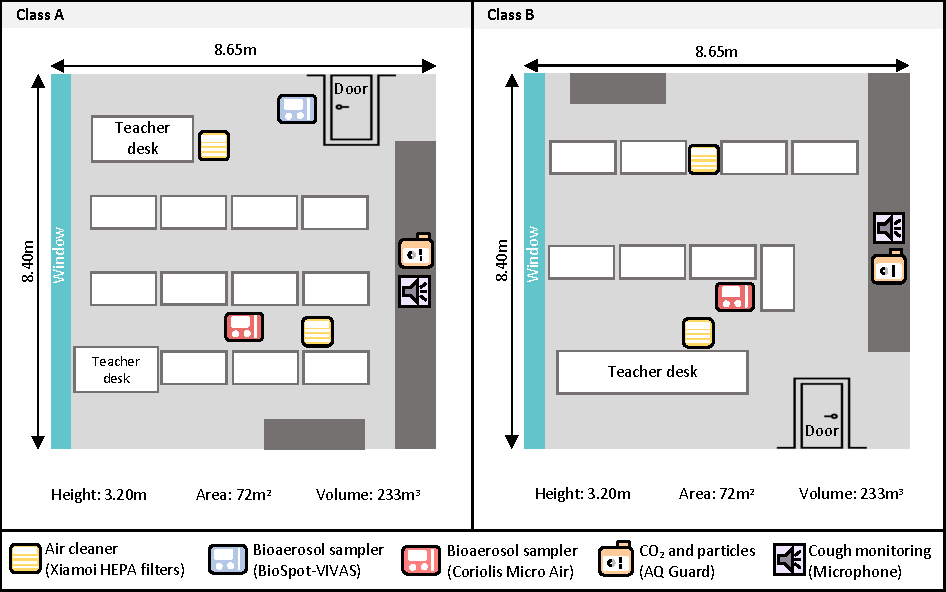
\includegraphics{../study_setting.pdf}
    \caption{\textbf{Study setting}. Schematic study setup of the classrooms. One air cleaner was placed in the front and the other in the back of classrooms. All devices were placed at the head level of students when they were seated. Both classrooms were not equipped with an active HVAC (Heating, Ventilation, Air conditioning) system, but were ventilated using passive window ventilation. }
    \label{fig:study-setup}
\end{figure}

\begin{table}[!htpb]
    \footnotesize
    \centering
    \caption{\textbf{Data}. Type of data collected, method/device, and frequency in the rooms of classes A and B.}
    \begin{tabular}{p{3.5cm}p{6cm} p{1cm} p{1cm} p{3cm}}
    \midrule
    Type of data & Method / device & Class A & Class B & Frequency \\
    \midrule
    \textbf{Molecular data} \\
    \midrule
    Bioaerosol sampling & Bioaerosol sampling devices: BioSpot-VIVAS (Aerosol Devices Inc., Ft. Collins, Colorado, United States) and Coriolis Micro Air (Bertin Instruments Montigny-le/Bretonneux, France) & x & (x) \newline only Coriolis & daily \\
    Saliva samples & Saliva samples & x & x & twice per week \\
    Swabs from air cleaners & Swab samples from Xiaomi HEPA filters (Xiaomi Mi Air Pro 70m2, Shenzhen, China) & x & x & after each intervention phase (both classes) and before the vacation (only class B) \\ 
    \midrule
    \textbf{Environmental data} \\
    \midrule
    CO$_2$, aerosol/particle concentrations, humidity, temperature & Air quality device: AQ Guard (Palas GmbH, Karlsruhe, Germany) & x & x & daily by minute \\
    Coughs & Sounds collected via microphones and coughs detected with a Machine Learning model \cite{Bertschinger2023CBMS} & x & x & daily by seconds \\
    \midrule
    \textbf{Epidemiological data} \\
    \midrule
    Absences & Survey & x & x & daily \\
    Student characteristics & Survey & x & x & at study start \\
    \bottomrule
    \end{tabular}
    \label{tab:data}
\end{table}

\subsection{Study intervention} 

\noindent We used a cross-over design to study the effectiveness of air cleaners, thereby distinguishing two study conditions in each class: weeks with and weeks without installation of air cleaners in the classroom (Fig.~\ref{tab:study-design}). Air cleaners refer to commercially available portable HEPA-filtration devices (Xiaomi Mi Air Pro 70m², Shenzhen, China; approx. USD\,250 per device), running at 2$\,\times\,$600 m$^{3}$/h clean air delivery rate. Passive window ventilation occurred per recommendations by the national public health authorities during both study conditions.

\begin{table}[!htpb]
    \footnotesize
    \centering
    \caption{\textbf{Study design.} Cross-over design where two portable air cleaners (AC) were installed during different time periods in classes A and B over a seven-week study period from 16~January to 11~March 2023, excluding a week of vacation between February 6 and 11.}
    \begin{tabular}{l l l l l l l l l}
    \toprule
      & \textbf{Week 1} & \textbf{Week 2} & \textbf{Week 3} & Vacation & \textbf{Week 4} & \textbf{Week 5} & \textbf{Week 6} & \textbf{Week 7} \\
      & Jan 16-21 & Jan 23-28 & Jan 30-Feb 3 & Feb 6-11 & Feb 13-18 & Feb 20-25 & Feb 27-March 3 & March 6-11 \\
      \midrule
      \textbf{A} & \cellcolor{gray!50} AC & \cellcolor{gray!50} AC & \cellcolor{gray!10} None & & \cellcolor{gray!10} None & \cellcolor{gray!10} None & \cellcolor{gray!50} AC & \cellcolor{gray!50} AC \\
      \textbf{B} & \cellcolor{gray!10} None & \cellcolor{gray!10} None & \cellcolor{gray!50} AC & & \cellcolor{gray!50} AC & \cellcolor{gray!50} AC & \cellcolor{gray!10} None & \cellcolor{gray!10} None \\
      \bottomrule
    \end{tabular}
    \label{tab:study_design}
\end{table}
 
\subsection{Data collection}

\noindent\textbf{Epidemiological data} \smallskip

\noindent At baseline, we collected aggregated data on age, sex and COVID-19 vaccination and recovery status in the participating classes. Daily we collected data on each absent student, \ie the absence, symptom onset and return date as well as the reason for the absence (sickness, career days,  or other) and symptoms. We also collected data on laboratory tests but none of the students reported a test result over the study. Based on the epidemiological data, we defined a case of respiratory infection as an absence where the student reported a sickness with at least one of the following symptoms: fever, coughing, tiredness, loss of test or smell, sore throat, headache, aches and pains, diarrhea, difficulty breathing or shortness of breath, stomach. Students were asked to report the first date when they experienced symptoms, \eg a student absent on Monday may report Saturday or Sunday as the symptom onset date. We will denote cases by their symptom onset date. Note that, during the week, the symptom onset date will usually correspond to the absence date, unless the student went to school despite experiencing symptoms. The line list data is shown in \supp~\zref{sec:case-data}. Informed consent of one student could not be obtained and his/her one absence was considered as unrelated to a respiratory infection. Reports about absences were entered electronically into a REDcap database\cite{Harris2009,Harris2019}. Furthermore, both classes participated in repetitive bi-weekly (Tuesdays and Thursdays) testing for a panel of respiratory infections (see \nameref{sec:mol_analyses} below). The saliva samples were transported to the laboratory and stored at $-$80°C until further processed\cite{Galar2021,To2019,Huber2021}. \medskip

\noindent\textbf{Environmental data} \smallskip

\noindent \emph{CO$_2$ and particle measurements} 

\noindent An air quality device (AQ Guard, Palas GmbH, Karlsruhe, Germany) continuously measured indoor CO$_2$ levels, aerosol number concentrations (particle diameter between 175~nm to 20~$\mu$m) and particle mass concentrations (PM; PM$_1$, PM$_{2.5}$, PM$_4$, PM$_{10}$) by minute. A transient mass balance model was used to estimate the air change rate from indoor CO$_2$ levels\cite{Batterman2017IJERPH}, assuming that the classrooms were fully occupied during lessons and that room occupancy increased (decreased) linearly 10~minutes before (after) the start (end) of a class. Particle concentrations were filtered according to the times students were in the classroom, which were monitored together with the time windows were opened. \medskip

\noindent \emph{Bioaerosol sampling} 

\noindent We collected airborne respiratory viruses in the classroom with a bioaerosol sampling device (BioSpot-VIVAS, Aerosol Devices Inc., Ft. Collins, CO, USA). This device samples airborne virus particles into a viral transport medium (VTM) using a laminar flow water-based condensation method. In parallel, we also used the Coriolis Micro Air (Bertin Instruments Montigny-le-Bretonneux, France) sampler, running at 200\,l/min and collecting into 15\,mL PBS  as previously reported in clinic settings\cite{Moore2021}. BioSpot-VIVAS operated throughout lessons while Coriolis Micro Air only operated shortly before and during break times to reduce noise exposure (approximately 60\,min/day). The removable parts of both sampling devices were regularly autoclaved to avoid contamination. At the end of the day, samples were transported to the Institute of Infectious Diseases (IFIK) and stored at $-$80°C. At the end of the study period, the Xiaomi HEPA filters were carefully removed and 20\,swabs were taken from each filter and stored at $-$80°C until further processed. \medskip

\subsection{Laboratory and molecular analyses}\label{sec:mol_analyses}

\noindent Prior to the real-time (RT)-PCR analysis, daily bioaerosol samples were combined for each sampling device and filtered using Amicon Ultra-15 Centrifugal Filters with Ultracel 10,000 Dalton molecular weight cutoffs filters (UFC9010; MilliporeSigma, Burlington, USA) to a volume of 1\,mL. The human saliva samples were directly analyzed without prior filtration. The Allplex RV Master Assay (Seegene, Seoul, South Korea) detects a panel of 19~respiratory viruses: SARS-CoV-2, Influenza A virus, Influenza B virus, Human respiratory syncytial virus A/B (RSV), Human metapneumovirus (MPV), Human adenovirus A/B/C/D/E/F (AdV), Human rhinovirus A/B/C (HRV), and Human parainfluenza virus 1/2/3/4 (PIV) in one single reaction. Viral genome load (VGL) of specimens was quantified (copies/L) by curve extrapolation derived from standardized ATCC quantitative genomic standard dilutions (ATCC-VR-3347D, LGC Standards, LGC Group UK). For the BioSpot-VIVAS air samples, the air concentration of the DNA was exactly calculated according to the airflow influx into the sampling device. The Limit of detection (LOD) of the assay SARS-CoV-2, IFA/IFB is 7.5x10$^0$ TCID/ml (SARS-CoV-2), 3.7x10$^{-1}$ TCID/ml (IFA), and 4.8x100 TCID/ml (100cp/ml) (IFB) respectively. For positive samples, we performed targeted sequencing to compare genetic relatedness between SARS-CoV-2 strains detected in the air and human samples\cite{Goncalves2021}, but we were unable to amplify and sequence any of the gene targets in the bioaerosol samples due to low RNA concentrations. 

\subsection{Statistical analyses and modeling}

All statistical analyses were described in the statistical analysis plan (SAP)\cite{Banholzer2023SAP}, which was published before analyses began. In contrast to the SAP, the number of positive bioaerosol samples and the viral load concentration of positive samples could not be analyzed because there were too few positive samples over the study. Apart from that there were no major deviations from the SAP regarding the conducted analyses. There were a few minor deviations from the SAP (\eg small changes in prior distributions or model specifications), which are documented in \supp~\zref{sec:transmission-model} to \supp~\zref{sec:env-regression-model}, which provide detailed descriptions of the models used in each analysis.

\noindent\textbf{Risk of infection} \smallskip

\noindent We estimated the relative risk of infection with air cleaners using a Bayesian latent hierarchical regression model. The observed outcome of this model is the number of new respiratory cases $C$ (absences related to respiratory infections by date of symptom onset) on day $t$ in class $j$, which are modeled with a Negative Binomial distribution. The expected number of new cases is the weighted sum of the number of new infections $I_{js}$ (unobserved/latent outcome) in the previous days $s<t$, with the weights corresponding to the probability distribution of the incubation period. The number of new infections is related to the presence of air cleaners using a regression-like log-link
\begin{align}
    \log I_{js} = \log F_{js} - \log N_{js} + \beta_0 + \beta_1 \cdot \text{AirCleaner}_{js},
\end{align}
where $F_{js}$ is the number of infections in the previous week (a proxy for the number of infectious students), $N_{js}$ is the cumulative number of infections, $\beta_0$ is the infection rate without air cleaners, and $\beta_1$ is the effect of air cleaners. Furthermore, the effect of air cleaners is adjusted for class-specific effects, the number of students in class, the daily air change rate, and the weekly positivity rate for COVID-19 and the consultations for influenza-like illnesses in the community (\ie the Canton of Solothurn).

A detailed description of the model and choice of priors for all model parameters are provided in \supp~\zref{sec:transmission-model}. Importantly, since multiple pathogens were prevalent over the study period, we considered the distribution of the incubation period to be a weighted mix of the pathogen-specific distributions. The weights were inferred based on the proportion of positive saliva samples for each pathogen per week. As a result, the distribution of the incubation period used for modeling could change every week depending on the proportion of pathogens that were detected in the students' saliva. Moreover, respiratory cases by date of symptom onset were under-reported for weekends and thus a re-weighting scheme was used to account for weekday effects. \medskip

\noindent\textbf{Number of positive saliva samples} \smallskip

\noindent Molecular analysis determined which saliva samples were positive for a respiratory pathogen. We analyzed the number of positive saliva samples with a Bayesian Multinomial logistic regression model (\supp~\zref{sec:multinomial-model}) where the expected number of positive samples for a pathogen was linked to the presence of air cleaners, adjusting for class-specific effects and the number of susceptibles for each pathogen. The latter was computed as the difference between the number of students per class and the cumulative number of positive samples. As a sensitivity analysis, we lagged the test results by one test date (\ie from Tuesday to last Thursday and from Thursday to Tuesday) and one test week (\ie from Tuesday to last Tuesday and Thursday to last Thursday), to consider the unknown delay when students were infected and tested positive. 

\noindent\textbf{Aerosol and particle concentrations} \smallskip

\noindent We computed the average concentrations per day and compared these between study conditions. We estimated the reduction in concentrations using Bayesian log-linear regression models (\supp~\zref{sec:env-regression-model}), adjusting for class and weekday effects, the number of students in class, the air change rate, and the cumulative number of respiratory cases. \medskip


\noindent\textbf{Software and model estimation} \smallskip

\noindent All analyses were performed in R software (version 4.2.0)\cite{RCoreTeam2022} and modeling in Stan (version 2.21.0)\cite{Carpenter2017}. Model parameters were estimated with a Bayesian approach. Specifically, Markov chain Monte Carlo (MCMC) sampling was used as implemented by the Hamiltonian Monte Carlo algorithm with the No-U-Turn Sampler (NUTS)\cite{Hoffman2014}. Each model is estimated with 4 Markov chains and 2,000 iterations of which the first 1,000 iterations are discarded as part of the warm-up. Estimation power is evaluated via the effective sample size ESS and convergence of the Markov chains is evaluated with the Gelman-Rubin convergence diagnostic ($\hat{R}$). If not stated otherwise, we report posterior means and credible intervals (CrIs) based on the 50\%, 80\%, and 95\% quantiles of the posterior samples, respectively. The code is available from \url{https://osf.io/38j9g}.

% \subsection{Additional data collection} 

% \noindent We also collected data about the students' subjective experiences of well-being and emotions using standardized daily online questionnaires and a pre-post questionnaire\cite{Brandenberger2018}. These data are not part of the current analysis. 

\subsection{Ethics statement}

\noindent The Ethics Committee of the Canton of Bern, Switzerland, approved the study (reference no. 2021-02377). For the saliva samples, we included all students who were willing to participate and obtained written informed consent from their caregivers.


\newpage

\section{Results}

The study population consisted of 90~students (39~female, 51~male; Table~\ref{tab:cases-overview-school}). Of these, 27~students were fully vaccinated and 34~students had recovered from an infection within the last year. Over the seven-week study period (3,150 student-days in total), students were absent from school for 644~days (20\% of total) of which 147~days (23\% of absences) were due to isolation related to COVID-19, and 247~(38\% of absences) were due to sickness. Overall, there were 35~confirmed and 73~suspected cases of COVID-19, exceeding the number of students in some classes (Table~\zref{tab:cases-overview}). This suggests that only a proportion of suspected cases were actual cases of COVID-19 as it is unlikely that students were infected twice. We estimated 55 (95\%-CrI 35 to 76) cases of COVID-19 across schools. \deleted{(\supp~Fig.~\zref{fig:redcap-supp-total-cases}).} 

\begin{table}[!htpb]
    \centering
    \caption{Overview of the study population, number of COVID-19 cases, and person-days of absences.}
    \label{tab:cases-overview-school}
    \footnotesize
    \begin{tabular}{l r r r}
    \toprule
         &  School 1 & School 2 & Total \\ \midrule 
        \textbf{Students} & \textbf{52 (58\%)} & \textbf{38 (42\%)} & \textbf{90 (100\%)} \\
        \emph{Gender} \\
        $\drsh$ Female & 20 (38\%) & 19 (50\%) & 39 (\hphantom{0}43\%) \\
        $\drsh$ Male & 32 (62\%) & 19 (50\%) & 51 (\hphantom{0}57\%) \\
        \emph{Vaccination status} \\
        $\drsh$ Vaccinated & 16 (31\%) & 11 (29\%) & 27 (\hphantom{0}30\%) \\
        $\drsh$ Not vaccinated & 36 (69\%) & 27 (71\%) & 63 (\hphantom{0}70\%) \\
        \emph{Recovery status} \\
        $\drsh$ Recovered last year & 25 (48\%) & 9 (24\%) & 34 (\hphantom{0}38\%) \\
        $\drsh$ Not recovered & 27 (52\%) & 29 (76\%) & 56 (\hphantom{0}62\%) \\
        & \\
        \textbf{Absent person-days} & \textbf{334 (52\%)} & \textbf{310 (48\%)} & \textbf{644 (100\%)} \\
        $\drsh$ Isolation & 109 (33\%) & 38 (12\%) & 147 (\hphantom{0}23\%) \\
        $\drsh$ Sickness & 95 (28\%) & 152 (49\%) & 247 (\hphantom{0}38\%) \\
        $\drsh$ Quarantine & 55 (17\%) & 5 (\hphantom{0}2\%) & 60 (\hphantom{00}9\%) \\
        $\drsh$ Other & 75 (22\%) & 115 (37\%) & 190 (\hphantom{0}30\%) \\
        & \\
        \textbf{COVID-19 cases} & \textbf{78 (19\%)} & \textbf{30 (13\%)} &  \textbf{108 (100\%)} \\
        $\drsh$ Confirmed & 25 (32\%) & 10 (\hphantom{0}33\%) & 35 (\hphantom{0}32\%) \\
        $\drsh$ Suspected & 53 (68\%) & 20 (\hphantom{0}67\%) & 73 (\hphantom{0}68\%) \\
        \bottomrule
    \end{tabular} 
\end{table}

\subsection{Molecular analyses}

We analyzed 262 saliva, 130 bioaerosol samples and swabs from the filters of air cleaners (20~swabs per filter) in two classrooms. We detected SARS-CoV-2, adenovirus, and influenza virus (Table~\ref{tab:molecular-data} and \supp~Table~\zref{tab:mol-data-1}-\zref{tab:mol-data-2}). SARS-CoV-2 made up the vast majority of positive saliva (19 out of 21) and bioaerosol samples (9 out of 10). We found four positive air-saliva samples in the same respective week (three SARS-CoV-2 and one adenovirus), suggesting they were paired samples. We also detected SARS-CoV-2 and influenza viruses from the HEPA filters of the air cleaners. The number of positive saliva and airborne SARS-CoV-2 samples per week varied by study condition (Fig.~\ref{fig:molecular-descriptives}a). Without interventions, the proportion of positive samples per week was 11.5\% for saliva and 8.1\% for airborne samples. These proportions were lower with mask mandates (Saliva: 5.7\%, Air: 7.1\%) and air cleaners (Saliva: 7.7\%, Air: 5.0\%). There were also differences in viral concentration in positive airborne samples (Fig.~\ref{fig:molecular-descriptives}b). Without interventions, it was 1.1\,copies per liter per week, which was higher than with mask mandates (0.7\,copies/L per week) and air cleaners (0.1\,copies/L per week). 

\begin{table}[!htpb]
    \centering
    \caption{\textbf{Analysis of molecular data}. Number of positive and negative saliva and airborne samples in each school.}
    \label{tab:molecular-data}
    \footnotesize
    \begin{tabular}{l rlrl p{.2cm} rlrl p{.2cm} rlrl}
    \toprule
    & \multicolumn{4}{c}{Saliva} & & \multicolumn{4}{c}{Air} & & \multicolumn{4}{c}{Air cleaner (HEPA filter)$^\dag$} \\ \cline{2-5} \cline{7-10} \cline{12-15} 
    & \multicolumn{2}{c}{School 1} & \multicolumn{2}{c}{School 2} & &  \multicolumn{2}{c}{School 1} & \multicolumn{2}{c}{School 2} & & \multicolumn{2}{c}{School 1} & \multicolumn{2}{c}{School 2} \\
    \midrule
    \textbf{Total} & \textbf{173} & & \textbf{89} & & & \textbf{68} & & \textbf{62} & & &  & &  & \\
    Negative & 160 & (\hphantom{0}92\%) & 81 & (\hphantom{0}91\%) & & 64 & (\hphantom{0}94\%) & 56 & (\hphantom{0}90\%) & &  & &  & \\  
    Positive & 13 & (\hphantom{00}8\%) & 8 & (\hphantom{00}9\%) & & 4 & (\hphantom{00}6\%) & 6 & (\hphantom{0}10\%) & & & &  & \\
    \midrule
    \textbf{Positive} & \textbf{13} & & \textbf{8} &  & & \textbf{4} & & \textbf{6} & & & \multicolumn{2}{l}{\textbf{2}}  & \multicolumn{2}{l}{\textbf{6}} \\
    SARS-CoV-2 & 12 & (\hphantom{0}92\%) & 7 & (\hphantom{0}88\%) & & 4 & (100\%) & 5 & (\hphantom{0}83\%) & & 2 & (100\%) & 4 & (\hphantom{0}66\%) \\
    Influenza & 1 & (\hphantom{00}8\%) & 0 & (\hphantom{00}0\%) & & 0 & (\hphantom{00}0\%) & 0 & (\hphantom{00}0\%) & & 0 & (\hphantom{00}0\%) & 1 & (\hphantom{0}17\%) \\
    Adeno & 0 & (\hphantom{00}0\%) & 1 & (\hphantom{0}12\%) & & 0 & (\hphantom{00}0\%) & 1 & (\hphantom{0}17\%) & & 0 & (\hphantom{00}0\%) & 1 & (\hphantom{0}17\%) \\
    \bottomrule
    \multicolumn{15}{l}{\scriptsize \emph{$\dag$: 20 swabs were taken from each filter at the end of the study period.}}
    \end{tabular}
\end{table}

\begin{figure}[!htpb]
    \centering
    \includegraphics{figures/molecular-descriptives.pdf}
    \caption{\textbf{Analysis of molecular data and comparison by study condition}. \textbf{(a)}~Proportion of positive airborne (solid line) and saliva (dashed line) samples (average per week). \textbf{(b)}~Viral concentration in positive airborne samples from BioSpot-VIVAS (average per week).}
    \label{fig:molecular-descriptives}
\end{figure}

\subsection{Analysis of aerosol and particle concentrations}

Particle concentrations differed by study condition (Fig.~\ref{fig:palas-results}a). Aerosol number concentrations were lower with mask mandates (49$\pm$52\,1/cm$^3$) and air cleaners (84$\pm$56\,1/cm$^3$) than without interventions (177$\pm$109\,1/cm$^3$). Similarly, particle mass concentrations (\eg PM$_1$) were lower with mask mandates (2.0$\pm$1.6\,$\mu$gm$^{-3}$) and air cleaners (3.8$\pm$2.9\,$\mu$gm$^{-3}$) than without interventions (6.9$\pm$4.1\,$\mu$gm$^{-3}$). CO$_2$ levels without interventions (953$\pm$198\,ppm) were slightly lower than with mask mandates (1,155$\pm$237\,ppm) and air cleaners (1,088$\pm$224\,ppm), indicating increased ventilation through outdoor air exchange (\supp~Fig.~\zref{fig:palas-supp-descriptives}), although the proportion of times windows were opened did not change with mask mandates (0.03, 95\%-CrI $-$0.07 to 0.12) or air cleaners (0.00, 95\%-CrI $-$0.11 to 0.11). When adjusting for different ventilation rates, the number of students in class, school and weekday effects, the aerosol number concentration decreased by 69\% (95\%-CrI 42\% to 86\%) with mask mandates and by 39\% (95\%-CrI 4\% to 69\%) with air cleaners (Fig.~\ref{fig:palas-results}b and Table~\zref{tab:palas-est-results}). The concentration of smaller particles (PM$_1$ and PM$_{2.5}$) was more reduced by mask mandates and the concentration of larger particles (PM$_4$ and PM$_{10}$) was more reduced by air cleaners. 

\begin{figure}[!htpb]
\centering
    \includegraphics[width=\linewidth]{figures/palas-descriptives.pdf}
    \includegraphics[width=\linewidth]{figures/palas-results.pdf}
    \caption{\textbf{Analysis of particle concentrations and comparison by study condition}. \textbf{(a)}~Boxplot of the daily average values for aerosol number concentration (CN in 1/cm$^3$) and particle mass concentration (PM for particles of sizes <1 to <10~$\mu$m, respectively in $\mu$gm$^{-3}$). Results for CO$_2$ and other environmental variables are shown in \supp~\zref{sec:detailed-palas}. \textbf{(b)}~Estimated reduction in aerosol number and particle mass concentrations with interventions (posterior mean as dot and 50\%-, 80\%- and 95\%-CrI as lines, respectively). }
    \label{fig:palas-results}
\end{figure}

\subsection{Estimating transmission risk of SARS-CoV-2}

The cumulative number of cases of COVID-19 increased considerably in all classes without intervention and the large majority of students has been infected in School~1 by the time air cleaners were installed, except for class~D in School~2 (Fig.~\ref{fig:redcap-results}a).  Based on our Bayesian transmission model, the probability of getting infected was lower with mask mandates than without interventions (adjusted odds ratio 0.19, 95\%-CrI 0.09 to 0.38) and comparable with air cleaners (1.00, 95\%-CrI 0.15 to 6.51). Accordingly, mask mandates were associated with a considerable number of avoided infections (9.98, 95\%-CrI 2.16 to 19.00), but not air cleaners (Fig.~\ref{fig:redcap-results}b). As an additional analysis, we used a modified Wells-Riley equation\cite{Rudnick2003} and assumed that the change in the rate of emitted infectious quanta were proportional to the \replaced{estimated}{measured} reduction \added{mean and 95\%-CrI) in the aerosol number concentration, while other parameters were kept constant under all study conditions (\supp~\zref{sec:transmission-risk}). Accordingly, the daily risk of infection for a six~hour school day was 1.0\% (95\%-CrI 0.4\% to 1.9\%) with mask mandates and 1.9\% (95\%-CrI 1.0\% to 3.0\%) with air cleaners, compared with a 3.1\% risk \added{for the baseline} without interventions (\supp~Fig.~\zref{fig:results-trans-risk}).

\begin{figure}[!htpb]
    \includegraphics[width=\linewidth]{figures/redcap-descriptives.pdf} 
    \includegraphics[width=\linewidth]{figures/redcap-results.pdf}
    \caption{\textbf{Analysis of epidemiological data and estimated transmission by study condition using Bayesian hierarchical transmission model}. \textbf{(a)}~Estimated mean cumulative number of cases for each school class after probabilistic simulation accounting for uncertainty in suspected cases and the date of symptom onset (\supp~\zref{sec:prob-sim}). Dotted red lines indicate the number of students per class. A comparison of the estimated number of new cases after probabilistic simulation with the observed number of new confirmed and suspected cases is shown in \supp~Fig.\zref{fig:redcap-supp-descriptives}. \textbf{(b)}~Estimated number of avoided infections associated with interventions across schools (posterior mean as dot and 50\%, 80\%, and 95\%-CrI as shaded areas) based on Bayesian hierarchical transmission model. Detailed estimation results are shown in \supp~\zref{sec:detailed-redcap}.}
    \label{fig:redcap-results}
\end{figure}


\FloatBarrier

\newpage

\section{Discussion}

We collected epidemiological, environmental, and molecular data to estimate transmission of respiratory infections in schools and assessed the effectiveness of infection control measures. Airborne detection of SARS-CoV-2 documented sustained SARS-CoV-2 transmission. Bioaerosol SARS-CoV-2 concentrations with general mask mandates were lower, and SARS-CoV-2 was detected on the filters of air cleaners. Aerosol number and particle mass concentrations dropped significantly with both interventions. The Bayesian transmission model estimated that mask mandated avoided SARS-CoV-2 infections, but not air cleaners.

Our study demonstrated airborne detection of SARS-CoV-2 in schools. Although sampling and molecular detection of infectious bioaerosols are challenging and there is no agreed standard\cite{Santarpia2020,Morris2022,Stockwell2019}, it provides important evidence on the airborne transmission of respiratory pathogens. So far, viral RNA in airborne samples of SARS-CoV-2 was mainly found in hospitals and healthcare facilities\cite{Shen2021}. A related study in two South African schools detected airborne \emph{Mycobacterium tuberculosis}\cite{Bunyasi2022}. Tuberculosis was the leading cause of death worldwide due to an infectious disease prior to the COVID-19 pandemic. An improved understanding of airborne transmission and the effectiveness of interventions can benefit the control of both infectious diseases\cite{Rieder2021}. Our study provides evidence on airborne SARS-CoV-2 viral transmission and the potential effects of interventions in schools based on airborne and saliva samples from students. In our study, positive samples mostly pertained to SARS-CoV-2, but we occasionally detected other respiratory viruses such as adenovirus and influenza. General public health measures during the study likely suppressed the spread of other respiratory viruses. It also must be noted that the detected viral concentrations were low, as shown by high cycle thresholds (CTs) in the RT-qPCR results. The molecular presence of other viral pathogens cannot be excluded. The low sensitivity of molecular assays to detect airborne pathogens is a common challenge\cite{Morris2022,Stockwell2019}.

An experimental study demonstrated the effectiveness of infection control measures (universal face mask wearing and air cleaners) using simulated exhaled SARS-CoV-2 bioaerosols in a closed indoor space\cite{Lindsley2021}. In contrast, we studied infection control measures in a real-life setting and demonstrated their effectiveness using a multiple-measurement approach, and obtain similar results. Our findings also align with existing evidence from population-level studies showing that the incidence of COVID-19 was lower schools with mask use\cite{Heinsohn2022,Gettings2021} and improved ventilation\cite{Gettings2021}. Similarly, a field study showed that adequate ventilation was associated with reduced incidence of tuberculosis, a strictly airborne disease, in a university building\cite{Du2020}. Altogether, these findings support arguments in favor of multiple intervention strategies to address airborne transmission of respiratory infections in crowded indoor settings\cite{Morawska2021}. 

Indoor ventilation is one of the key determinants of airborne transmission\cite{Fennelly2020,Wang2021}, but schools are often poorly ventilated\cite{Santamouris2008,DiGilio2021}. We showed that air cleaners effectively reduce the concentration of both larger and smaller particles, in line with findings about their effectiveness in hospitals\cite{Morris2022} and simulated indoor environments\cite{Lindsley2021}. The detection of viruses on the filters of air cleaners further supports the evidence on the effective removal of bioaerosols. However, it was difficult to estimate changes in transmission following air cleaners because they were installed at the end of the study period when presumably a large proportion of students were already infected with SARS-CoV-2. In addition, physicochemical properties of aerosols, environmental factors and the distance to infectious people determine the survival of airborne particles and the loss of infectivity over time\cite{Wang2021}. Thus, a predominance of close range high particle density aerosol transmission of SARS-CoV-2 in school settings could further explain why air cleaners appeared not effective in preventing transmission. Our study used portable, affordable air cleaners that could be implemented at scale, rather than large cleaners\cite{Duill2021}. Noise exposure, and a lack of acceptance by teachers\cite{Sanguinetti2022} may still prevent their widespread use. Although not specifically assessed, we perceived good acceptance of our air cleaners during the short study period. Nevertheless, investments in professional building ventilation systems should be preferred to air cleaners in the long term\cite{Nardell2016}.  

School closures during the COVID-19 pandemic have been intensely debated as children and adolescents are particularly vulnerable to the negative impact of such interventions on their well-being and mental health\cite{Loades2020}. Furthermore, numerous studies have examined the role of children in transmitting SARS-CoV-2\cite{Goldstein2021} and it remains unclear to what extent transmission of SARS-CoV-2 occurs in schools\cite{Ulyte2021Clustering}. These findings contrast with studies of influenza viruses showing that school children may drive the seasonal influenza epidemic. Community studies in the US demonstrated that influenza transmission rates in children and adolescents were high in schools and that they easily transmit influenza viruses to household members and into their communities\cite{Glezen1978,Shang2018,Fiore2012}. Our study suggests that also transmission of SARS-CoV-2 occurs to a considerable extent in schools. 

Our study has several limitations. First, aerosol measurements and molecular detection of pathogens in bioaerosol samples document exposure, but not necessarily transmission and the direction of transmission (human to air, air to human) cannot be determined. Second, a comparison of viral concentration between study conditions should be interpreted with care due to the technical limitations of molecular detection in bioaerosol samples, and because the number of possibly infectious (and thus susceptible) students decreased towards the end of the study. Third, our epidemiological analysis is based on observational data, thus subject to potential confounding, \eg the incidence of COVID-19 (cases per week) in the community varied over the study period. However, levels were high throughout and included two Omicron subvariant peaks. Community transmission was also considered in our Bayesian transmission model. CO$_2$ levels were not considered in the model but the levels were slightly lower without interventions, suggesting that lower ventilation during intervention phases may have actually reduced the estimated effectiveness of mask mandates and air cleaners. Fourth, epidemiological data may not always be complete due to the under-reporting of COVID-19 among absent students. We thus used a probabilistic approach to estimate the proportion of suspected cases being actual cases of COVID-19 and the date of symptom onset where it was not reported. While this allows us to consider uncertainty in the observed data, the estimated effects of interventions will be less precise as reflected in the larger uncertainty intervals. 

In conclusion, using epidemiological, environmental, and molecular data, our study shows that considerable transmission of SARS-CoV-2 occurred in the participating schools. General face mask wearing were associated with reduced SARS-CoV-2 transmission and prevented infections. The effectiveness of interventions was supported by significant decreases in the concentration of aerosols. Taken together, our results suggests that infection control measures can reduce the transmission of respiratory infections in school rooms. Future studies may use our multiple-measurement approach to assess the effectiveness of infection control measures in reducing the transmission of respiratory infections. Ideally, these data should be collected routinely in sentinel schools, thus continuously monitoring transmission risks and alerting health authorities when infection control measures should be taken. 


\newpage


%TC:ignore
\section*{Acknowledgements}
We would like to thank the schools, teachers, and students participating in the study. We are also grateful to the Educational Department of the Canton of Solothurn for their support throughout the study. Finally, we are indebted to the student assistants who helped with the data collection at the schools.

\bibliography{references.bib}
%TC:endignore

\end{document}
